\documentclass[12pt]{beamer}


\usetheme[progressbar=frametitle]{metropolis}
\usepackage{appendixnumberbeamer}

\usepackage{booktabs}
\usepackage[scale=2]{ccicons}

%\usepackage{pgfplots}
%\usepgfplotslibrary{dateplot}

\usepackage{xspace}
\newcommand{\themename}{\textbf{\textsc{metropolis}}\xspace}

%\setbeamertemplate{footline} % To remove the footer line in all slides uncomment this line
%\setbeamertemplate{footline}[page number] % To replace the footer line in all slides with a simple slide count uncomment this line

%\setbeamertemplate{navigation symbols}{} % To remove the navigation symbols from the bottom of all slides uncomment this line


\usepackage{graphicx} % Allows including images
\usepackage{grffile}
\usepackage{amsmath}
\usepackage{adjustbox} 
\usepackage{tikz-cd}
 \usetikzlibrary{cd}
% have to have Mozilla's=Fira Sans} font and XeTeX installed to use full typography.

%----------------------------------------------------------------------------------------
%	TITLE PAGE
%----------------------------------------------------------------------------------------

\title{Alliances, Arms Transfers, and Electoral Trade Cycles}
\date{April 8, 2022}
\author{Joshua Alley}
\institute{Democratic Statecraft Lab, University of Virginia}


\begin{document}

 \maketitle


%----------------------------------------------------------------------------------------
%	PRESENTATION SLIDES
%----------------------------------------------------------------------------------------

%------------------------------------------------
% Here's my question. 
 \begin{frame}[standout]

U.S. political budget cycles expand international trade, especially arms exports to allies. 


 \end{frame}
 
 %------------------------------------------------

\begin{frame}{My Argument in Brief}

\begin{enumerate}
\item Political budget cycles increase trade.  
\pause 
\item Defense contracting has a critical role in budget cycles.
\pause 
\item Contracting cycles lead to arms exports, especially to allies. 
\pause
\item \textbf{Result}: General trade increase, and allies receive more U.S. exports than other states. 
\end{enumerate}

\end{frame}
 
  %------------------------------------------------

\begin{frame}{Why Should You Care?: Part 1}

%\begin{figure}[htbp]
%	\centering
%		\includegraphics[height=.95\textheight]{p-8a-poseidon.png}
%\end{figure}

% https://www.armscontrol.org/act/2018-04/news/trump-touts-saudi-arms-sales

\end{frame}
 
 %------------------------------------------------

\begin{frame}{Why Should You Care?: Part 2}

% maybe trump arms initiative and trade? Saudi photo
% juxtapose pressure on Powell to lower rates


\end{frame}


%------------------------------------------------

\begin{frame}{Outline}

\pause
\begin{enumerate}
\item Argument: Budget Cycles, Defense Contracting, Arms Transfers, and Trade. 
\pause
\item Results: Electoral Trade Cycles. 
\pause
\item Results: Defense Contracting and Arms Trade Cycles.  
\end{enumerate}


\end{frame}
 

%------------------------------------------------

\section{Argument} 

%-----------------------------------------------

\begin{frame}{Political Budget Cycles}

In order to win elections. 
\pause 
\begin{enumerate} 
\item Leaders use fiscal and monetary policy to increase economic growth. 
\pause 
\item Often targeted policies, such as defense contracting.
\end{enumerate}


\end{frame} 

%-----------------------------------------------

\begin{frame}{Economic Consequences of Budget Cycles}

\pause 
\begin{enumerate} 
\item Economic expansion increases domestic consumption.  
\pause 
\item Price effects of monetary expansion increase exports.
\pause
\item Imports and exports to all other countries rise. 
\end{enumerate}


\end{frame} 

%-----------------------------------------------

\begin{frame}{Defense Contracting and Arms Exports}

\pause 
\begin{enumerate} 
\item Presidents have more direct control over contract allocation.  
\pause 
\item Use this for targeted stimulus. 
\pause
\item Creates additional defense goods.
\pause
\item Some defense goods will be exported.
\end{enumerate}


\end{frame} 

%-----------------------------------------------

\begin{frame}{Arms Exports to Allies}

\pause 
\begin{enumerate} 
\item Allies provide a market for additional defense goods.
\pause 
\item Common security interests, defense industry integration. 
\pause
\item Doubles as commitment signal for U.S. leaders. 
\end{enumerate}


\end{frame} 

%-----------------------------------------------
%
%\begin{frame}[fragile]
%
%\pause 
%\begin{figure}[htpb]
%\adjustbox{scale = .55}{
%%\centering
%\begin{tikzcd}         
%  \mbox{Budget Cycles} \arrow[r] & \mbox{Defense Contracting} \arrow[r] & \mbox{Arms Exports} \arrow[r] & \mbox{Trade Cycles, especially arms to allies}   & 
%\end{tikzcd}
%}
%\end{figure}
%
%\end{frame} 

%-----------------------------------------------

\begin{frame}{Argument Summary}

\resizebox{.99\textwidth}{!}{
\begin{tabular}{ccccccc}
\mbox{Budget}  & $\rightarrow$    & \mbox{Defense}     & $\rightarrow$ & \mbox{Arms}     & $\rightarrow$ & \mbox{Trade Cycles} \\
\mbox{Cycles}  &                  & \mbox{Contracting} &               &  \mbox{Exports}   &               & \mbox{with Allies} \\
\end{tabular}
}


\end{frame}

%-----------------------------------------------

%------------------------------------------------

\section{Electoral Trade Cycles} 

%-----------------------------------------------

\begin{frame}{Research Design}

\pause
Analyze changes in US trade with all other states, 1951 to 2019. 
\pause
\begin{enumerate}
\item Outcome: Changes in log exports, imports, and total trade. Changes in trade balance.  
\pause
\item Independent Variables: Dummy indicator of defense alliance, years to presidential election.
\pause 
\item Estimator: Robust regression. 
\pause 
\item Adjust for gravity model factors, security threats, common interests, presidential partisanship.
\end{enumerate} 

\end{frame} 

%-----------------------------------------------

\begin{frame}{Electoral Trade Cycles}

\begin{figure}[htbp]
	\centering
		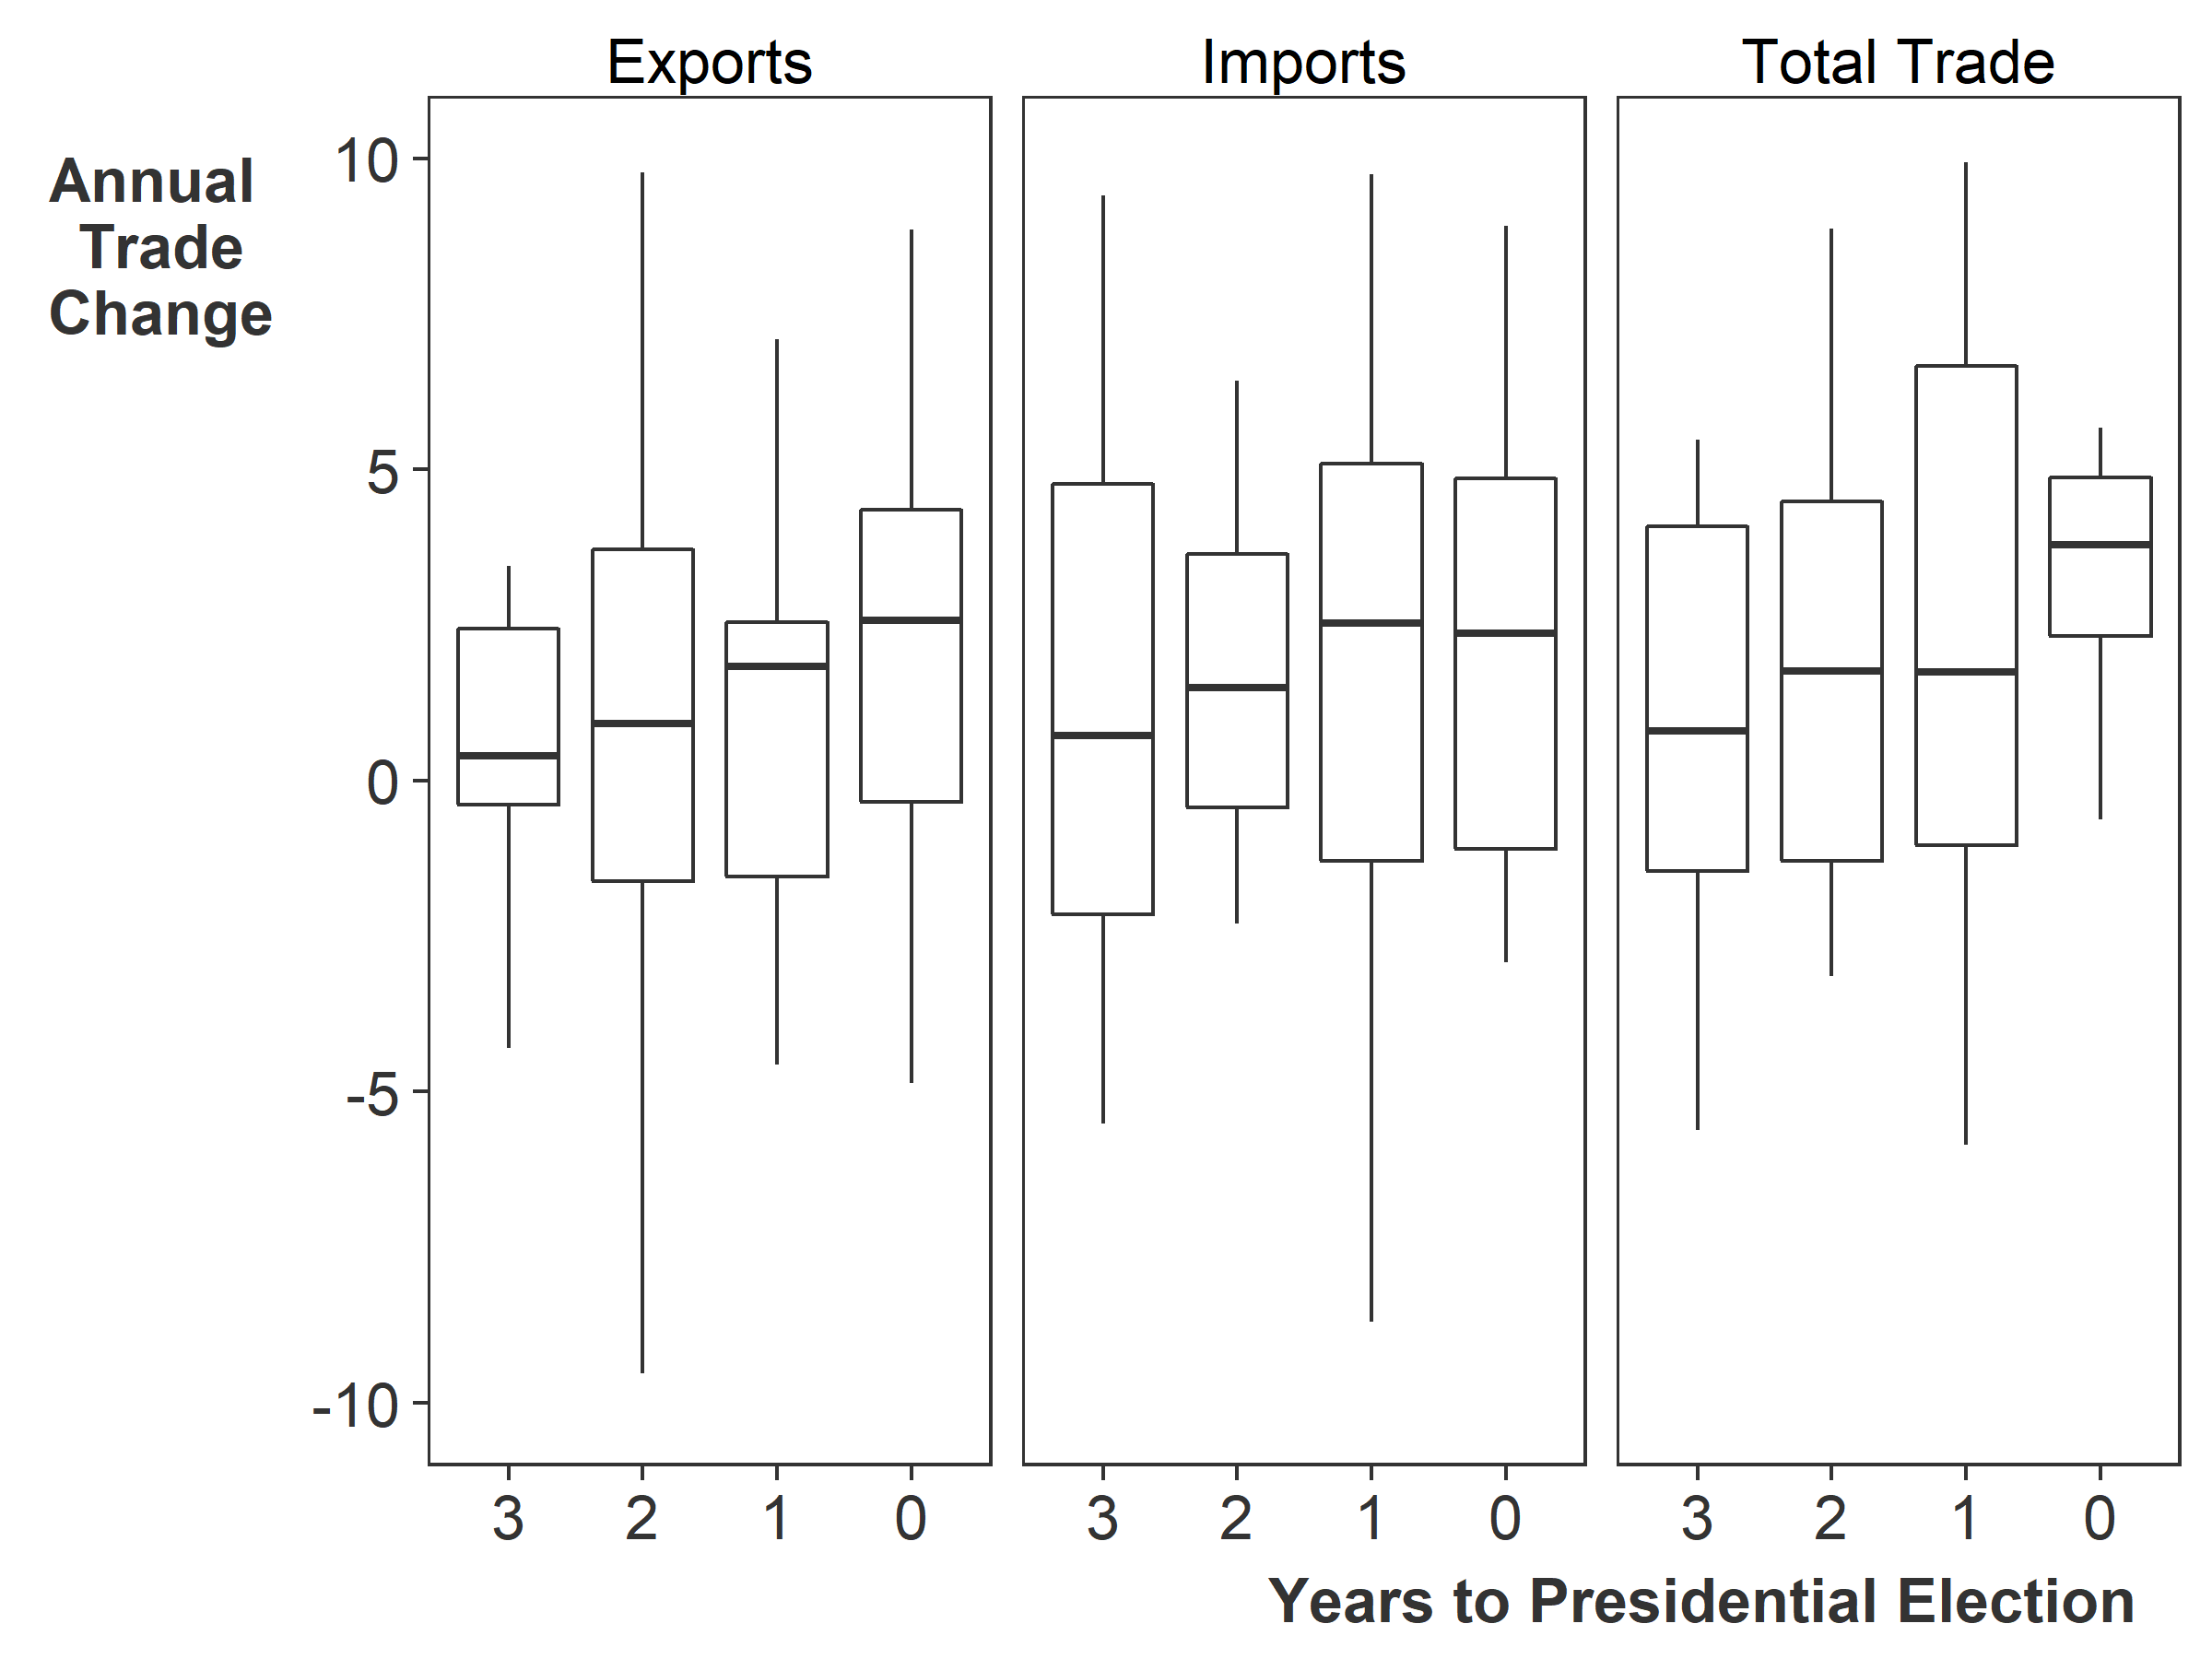
\includegraphics[height=.9\textheight]{us-trade-cycles.png}
\end{figure}


\end{frame} 


%-----------------------------------------------

\begin{frame}{Alliances and Trade Regression Results}

\begin{figure}[htbp]
	\centering
		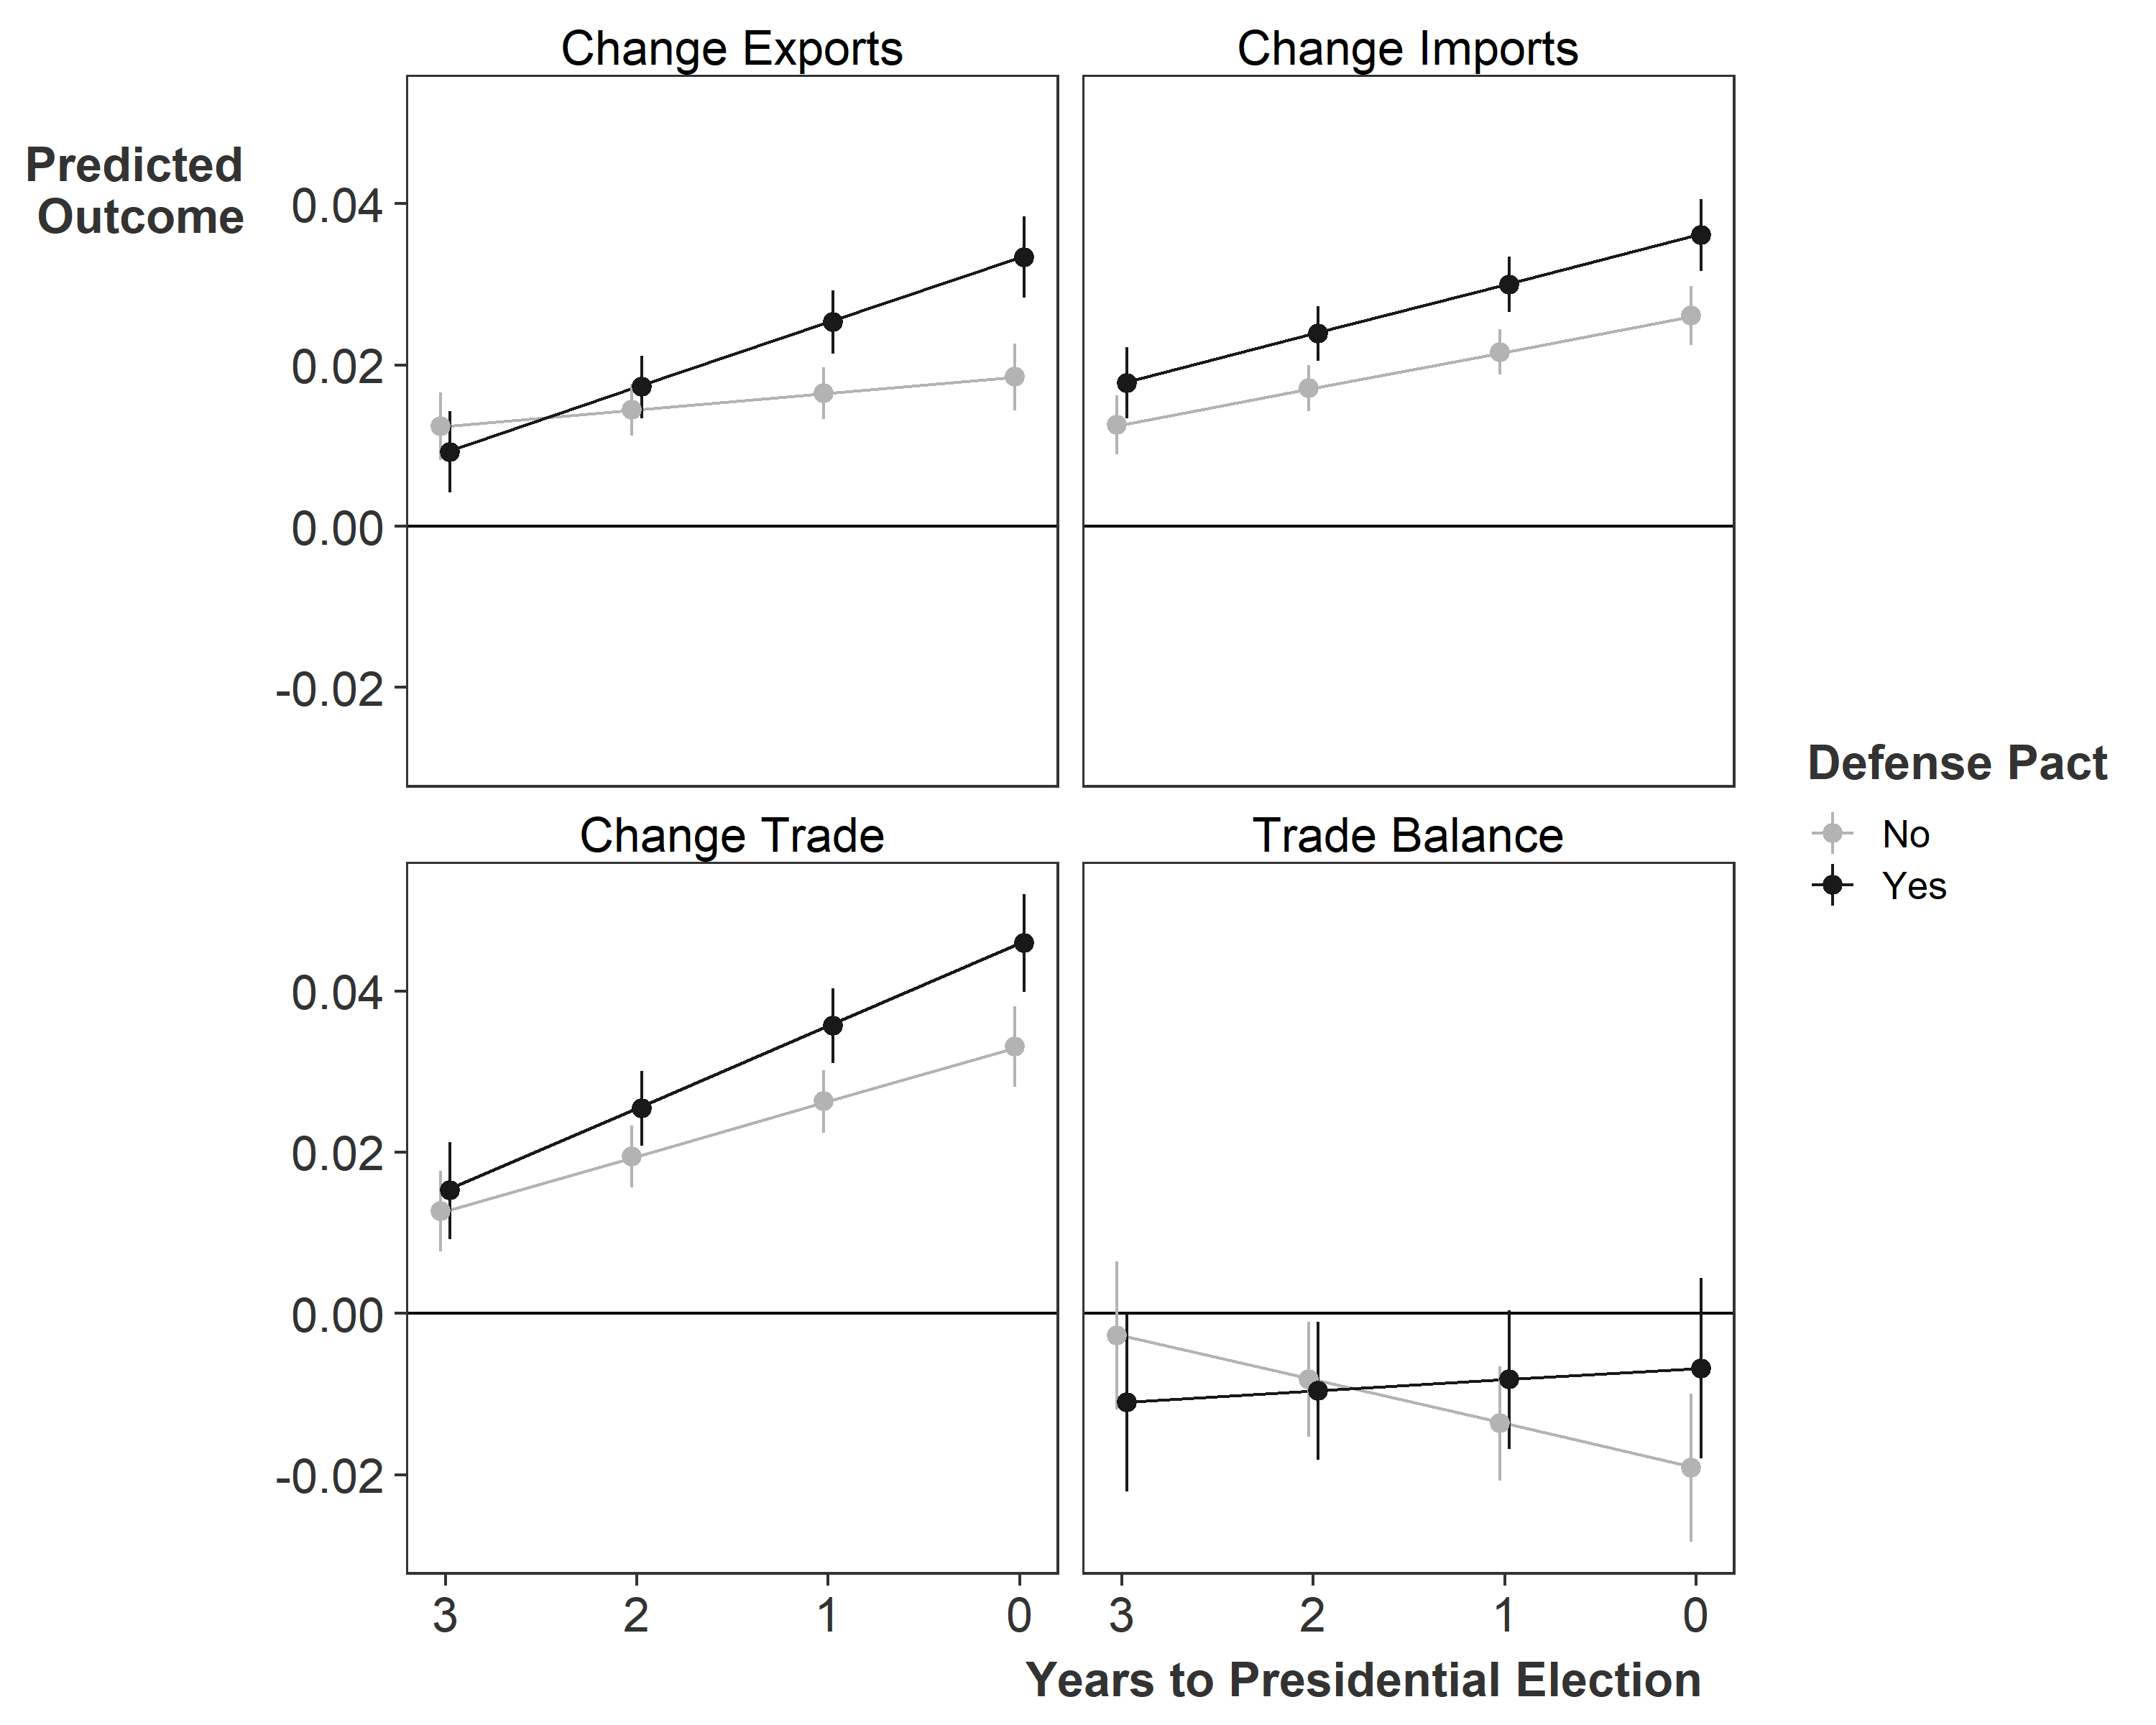
\includegraphics[height=.9\textheight]{us-elec-pred.png}
\end{figure}

\end{frame} 



%------------------------------------------------

\section{Defense Contracting and Arms Transfer Cycles} 

%-----------------------------------------------

\begin{frame}{Research Design}

\pause
Analyze US arms exports to all other states, 1951 to 2019. 
\pause
\begin{enumerate}
\item Outcome: Log Arms Transfers (SIPRI)
\pause
\item Independent Variables: Dummy indicator of defense alliance, years to presidential election.
\pause 
\item Estimator: Regression. 
\pause 
\item Adjust for trade model controls, lagged arms transfers, and non-zero arms transfer selection.
\end{enumerate} 

\end{frame} 

%-------------------------------------------------

\begin{frame}{Arms Exports, Alliances, and Elections}

\begin{figure}[htbp]
	\centering
		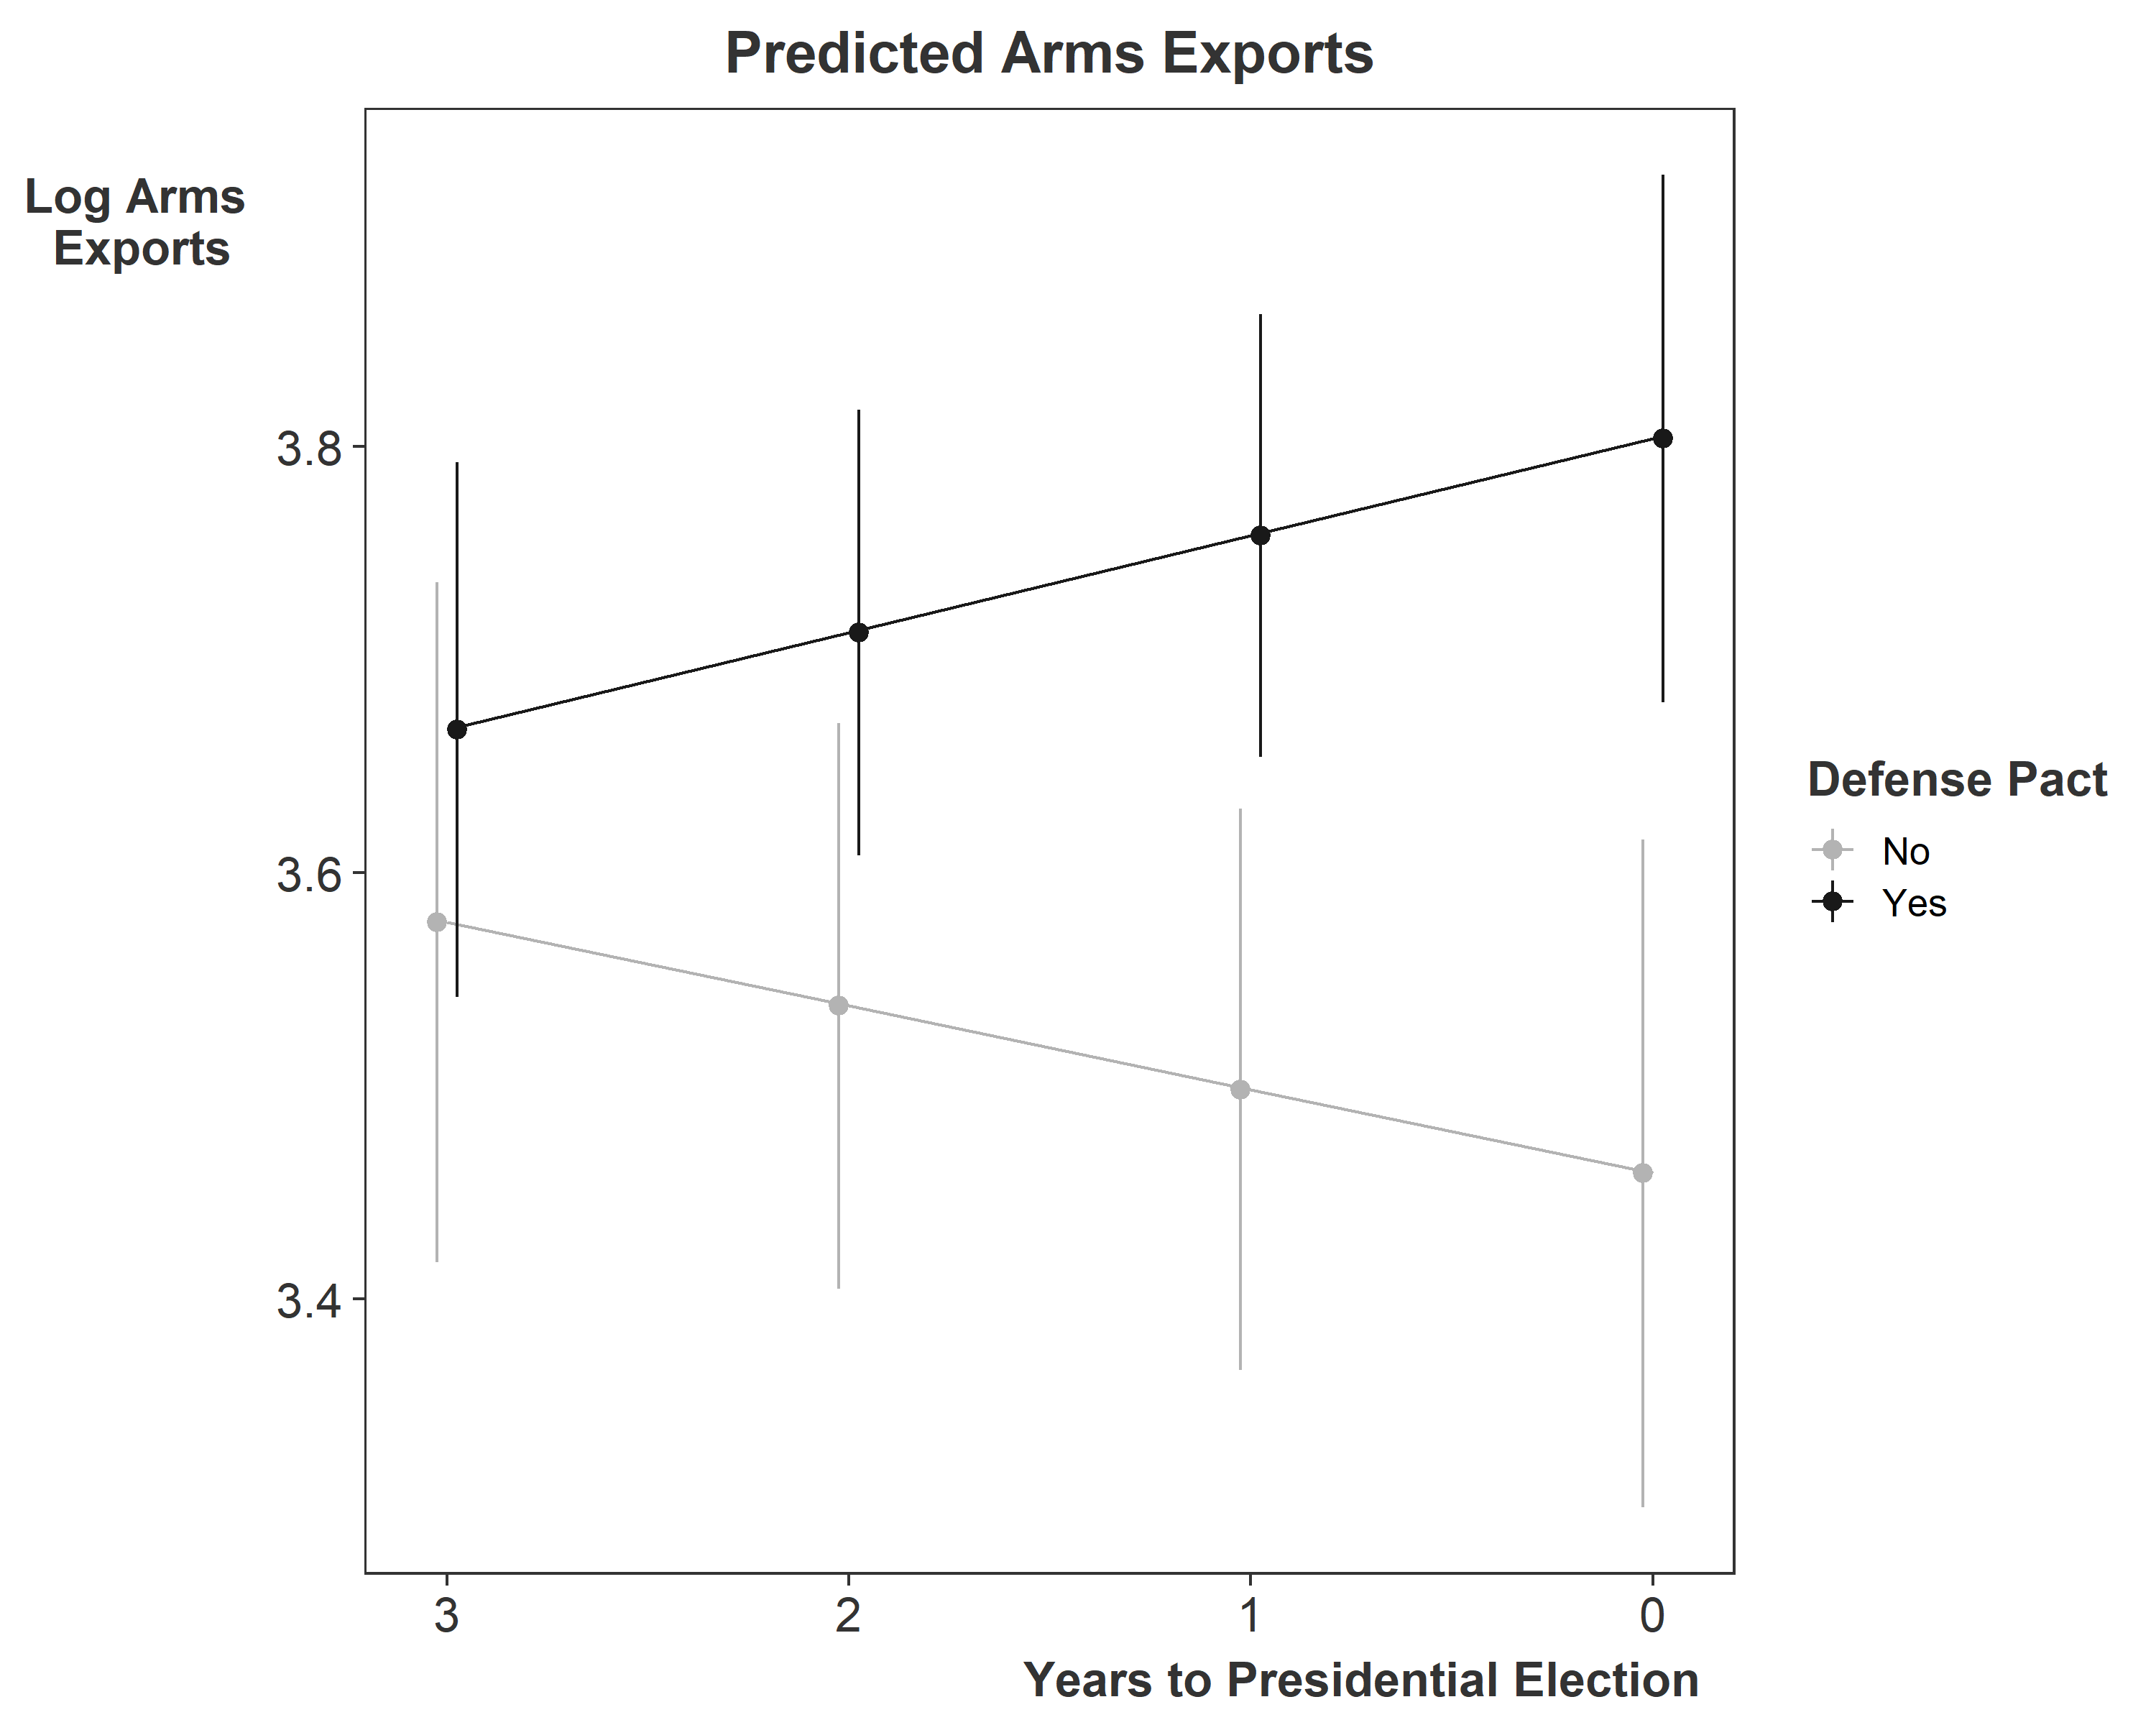
\includegraphics[height=.90\textheight]{us-arms-pred.png}
\end{figure}


\end{frame}


%-------------------------------------------------

\begin{frame}{Arms Exports, Alliances, and Elections}

\begin{figure}[htbp]
	\centering
		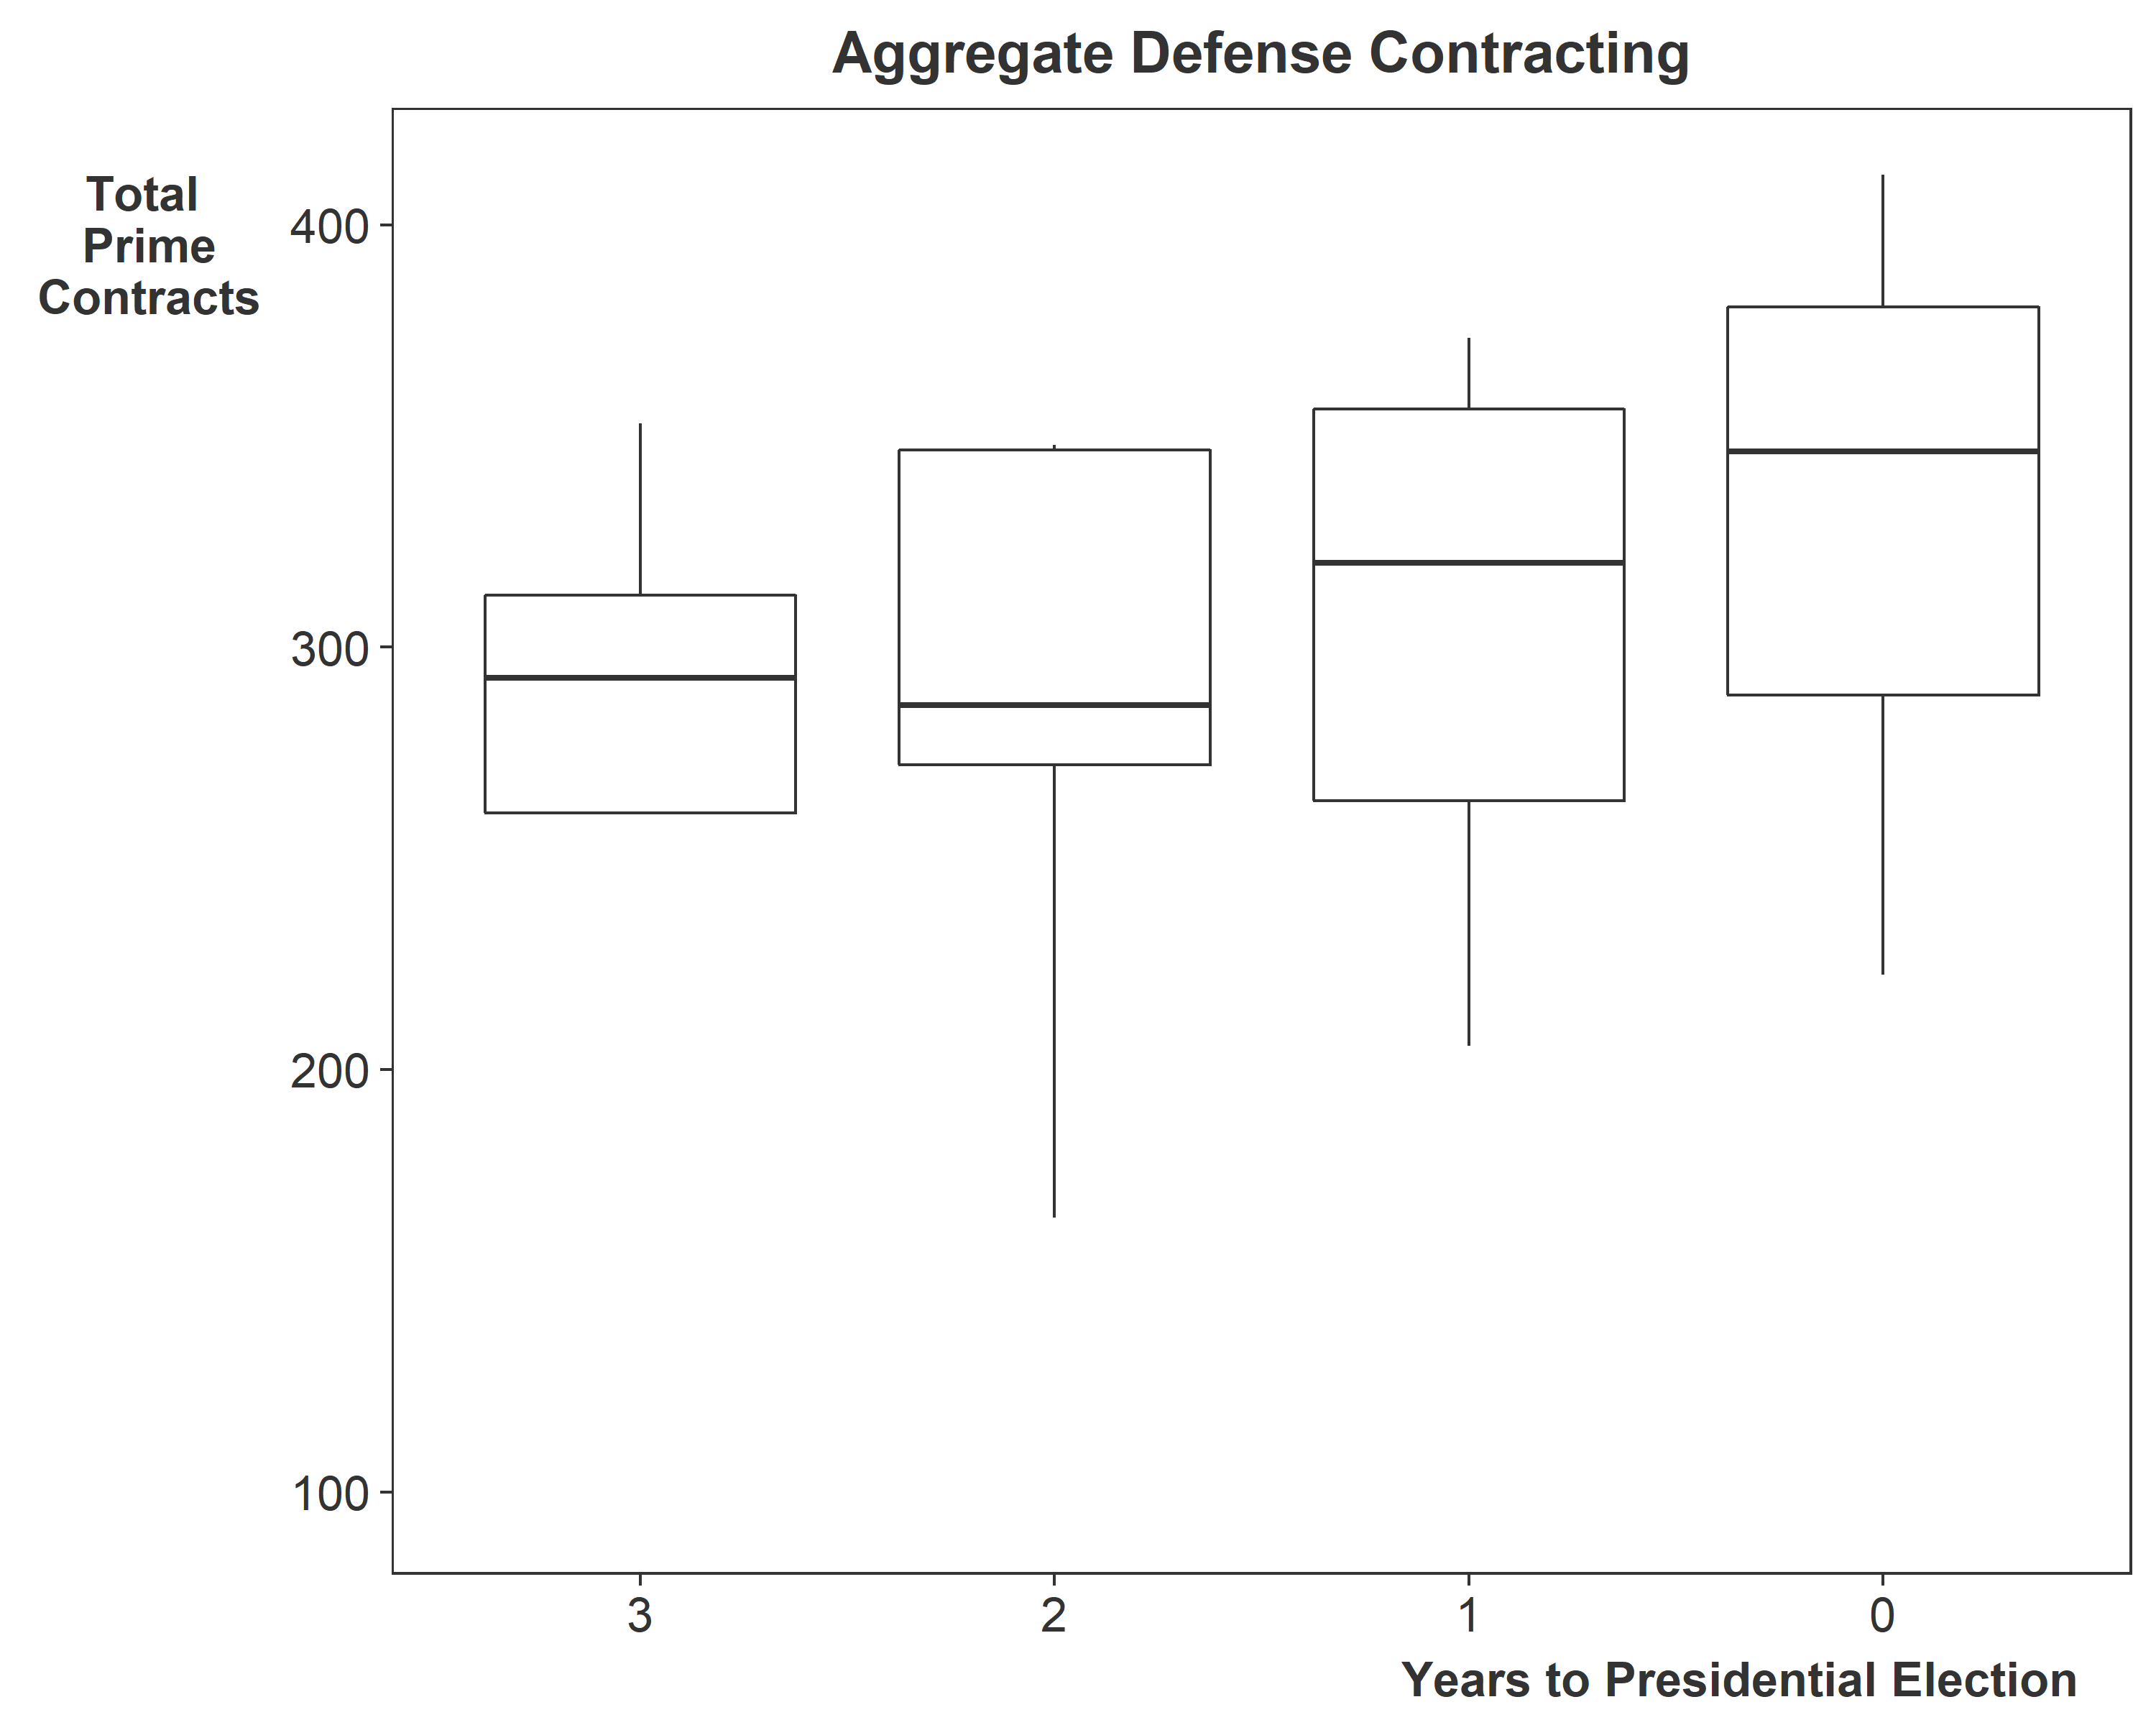
\includegraphics[height=.90\textheight]{contract-cycles.png}
\end{figure}


\end{frame}



%-----------------------------------------------


%------------------------------------------------

\section{Discussion and Conclusion} 

%-----------------------------------------------


\begin{frame}[standout]

U.S. political budget cycles expand international trade, especially arms exports to allies.  

\end{frame}


%------------------------------------------------
\begin{frame}{Discussion}

Some limitations. 

\pause
\begin{enumerate}
\item Could use more detailed trade data. 
\pause
\item Generalizing beyond the United States. 
\end{enumerate} 

\end{frame}


%%------------------------------------------------
\begin{frame}{My Research Agenda: Alliance Politics and Political Economy of Security}

\begin{columns}

% Major powers
\begin{column}{0.5\textwidth}
\textbf{Political Economy}
\begin{enumerate} 
\item Alliances and Military Spending: \textit{International Studies Quarterly}, \textit{Research \& Politics} and  \textit{Security Studies}.
\item Economic Consequences of Alliances: this project and economic benefits of US alliances. 
\end{enumerate} 
\end{column}


\begin{column}{0.5\textwidth}
\textbf{Political Economy of Civil Conflict}
\begin{enumerate}
\item Countering the Adaptable and Resilient: U.S. Foreign Terrorist Organization (FTO) List and Terrorist Attacks 
\item Conflict Management Institutions and Foreign Direct Investment in Post-Conflict States
\item Rumors of Boogaloo: Media and Support for Militant Right-Wing Extremism in the United States 
\end{enumerate} 
\end{column}


\end{columns}
 

\end{frame}

%-----------------------------------------------


%------------------------------------------------

\begin{frame}[standout]

Thank you! 

jkalley@virginia.edu

\end{frame}

%-----------------------------------------------

\appendix 

%-----------------------------------------------

%-----------------------------------------------

\begin{frame}{Elite Cues Attributes}


\end{frame}

%-----------------------------------------------




%----------------------------------------------------------------------------------------

\end{document}
